% 乘积拓扑
% 乘积拓扑|拓扑空间|笛卡儿积|拓扑基|子基|乘积映射

\pentry{拓扑空间\upref{Topol}}

\subsection{有限维乘积拓扑}

给定两个拓扑空间$(X_1, \mathcal{T}_1)$和$(X_2, \mathcal{T}_2)$,那么我们可以在乘积集合$X=X_1\times X_2$中定义一个拓扑$\mathcal{T}$,其拓扑基为$\{O_1\times O_2|O_1\in\mathcal{T_1}, O_2\in\mathcal{T_2}\}$.就是说,乘积集合的拓扑基,是两个空间中开集的笛卡尔积的集合.

\begin{figure}[ht]
\centering
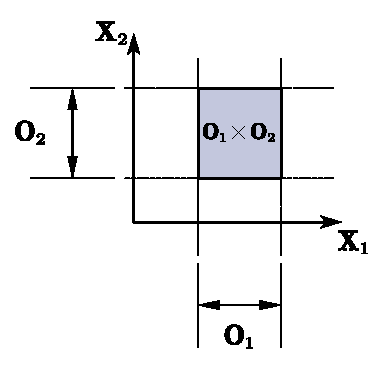
\includegraphics[width=6cm]{./figures/Topo6_2.pdf}
\caption{二维乘积拓扑的拓扑基中每个元素都是如图所示的一个“矩形”.} \label{Topo6_fig2}
\end{figure}

由拓扑基生成拓扑的方式(取任意并),容易发现,如果上述$O_1$和$O_2$取的只是$X_1$和$X_2$空间的某两个拓扑基,也能得到一样的定义.

一般地,$N$个拓扑空间的集合做笛卡尔积,这个笛卡尔积集合上的\textbf{乘积拓扑}定义为:

\begin{definition}{有限维乘积拓扑}
设$(X_n, \mathcal{T}_n)$是若干拓扑空间,$n$取值范围为$[1, N]\cap\mathbb{Z}$.那么乘积空间$X_1\times X_2\times X_3\times\cdots\times X_N=\prod\limits_{n=1,2,\cdots,N}X_n=X$中的拓扑由\textbf{拓扑基} $\mathcal{B}$生成,其中$\mathcal{B}=\{\prod\limits_{n=1,2,\cdots,N}O_n|\forall n, O_n\in\mathcal{T}_n\}$.
\end{definition}

\subsection{任意维乘积拓扑}

如果用于进行笛卡尔积的拓扑空间数量大于等于$\aleph_0$,那么我们常用的乘积拓扑定义会和有限维情况的说法略有不同.在这里,我们使用\textbf{子基(sub-basis)}来定义乘积拓扑:

\begin{definition}{任意维乘积拓扑}

设$(X_\alpha, \mathcal{T}_\alpha)$是若干拓扑空间,$\alpha$不再是整数指标,而是用一个集合$\Lambda$中的元素来表达的指标:$\alpha\in\Lambda$.这样的集合$\Lambda$称为一个\textbf{指标集(set of indexes)}.

空间$X=\prod\limits_{\alpha\in\Lambda}X_\alpha$的拓扑$\mathcal{T}$由\textbf{子基}$\mathcal{S}$生成,其中$\mathcal{S}=\{O_{\alpha_0}\times\prod\limits_{\alpha\in\Lambda-\{\alpha_0\}}X_\alpha|\alpha_0\in\Lambda, O_{\alpha_0}\in\mathcal{T}_{\alpha_0}\}$.就是说,$\mathcal{S}$中的每一个元素,都是某个$X_{\alpha_0}$的开集$O_{\alpha_0}$和其它所有$X_\alpha$乘积的结果.

\begin{figure}[ht]
\centering
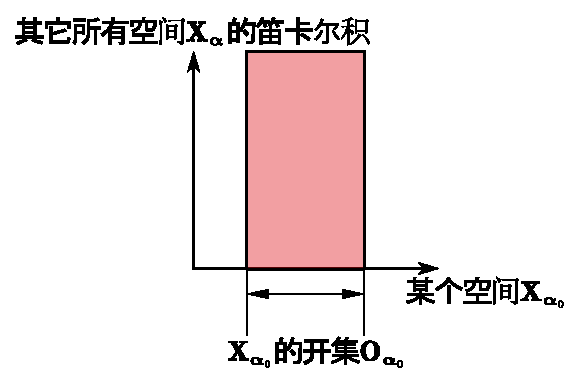
\includegraphics[width=7.5cm]{./figures/Topo6_1.pdf}
\caption{子基$\mathcal{S}$中的一个元素,类似一个“柱形”(类比$\mathbb{R}$空间之间的乘积).} \label{Topo6_fig1}
\end{figure}

其中,各$X_\alpha$空间称作$X$的一个\textbf{分量(component)},类比向量空间的称呼.

\end{definition}

任意维乘积拓扑也可以用拓扑基定义,只不过拓扑基中的元素不再是各分量空间的开集之乘积,而是有限个分量空间的开集和其它全体分量空间本身的乘积.

任意维乘积拓扑的定义是包含了有限维的定义的,因为当进行乘积的空间是有限个(即$|\Lambda|<\aleph_0$)的时候,任意维乘积拓扑的定义就和有限维乘积拓扑的定义一致了.

\subsection{乘积映射}

给定集合间的映射$f:A\rightarrow X$和$g:B\rightarrow Y$,可以定义映射$f\times g:A\times B\rightarrow X\times Y$.其中$\forall a\in A, b\in B$,有$f\times g(a, b)=(f(a), g(b))$.

\begin{exercise}{}\label{Topo6_exe1}
证明:如果上述集合是拓扑空间,并且$f$和$g$都是连续映射,那么$f\times g$也是乘积空间之间的连续映射.
\end{exercise}



